
\documentclass[10pt,
% a4paper,
%twocolumn,
fleqn,
%landscape, 
% papersize,
dvipdfmx,
uplatex
]{jsarticle}



\def\maru#1{\textcircled{\scriptsize#1}}%丸囲み番号

% \RequirePackage[2020/09/30]{platexrelease}

%太字設定
\usepackage[deluxe]{otf}

\usepackage{emathEy}

\usepackage[g]{esvect}

%大きな文字
\usepackage{fix-cm}

%定理環境
\usepackage{emathThm}
%\theoremstyle{boxed}
\theorembodyfont{\normalfont}
\newtheorem{Question}{問題}[subsection]
\newtheorem{Q}{}[subsection]
\newtheorem{question}[Question]{}
\newtheorem{quuestion}{}[subsection]

%セクション,大問番号のデザイン
\renewcommand{\labelenumi}{(\arabic{enumi})}
\renewcommand{\theenumii}{\alph{enumii})}
\renewcommand{\thesection}{第\arabic{section}章}

%用紙サイズの詳細設定
\usepackage{bxpapersize}
\papersizesetup{size={80mm,45mm}}
\usepackage[top=0.7zw,bottom=0truemm,left=3truemm,right=133truemm]{geometry}
\usepackage[dvipdfmx]{graphicx}

%余白など
\usepackage{setspace} % 行間
\setlength{\mathindent}{1zw}
\setlength\parindent{0pt}


%色カラーに関する設定
\usepackage{color}
\definecolor{shiro}{rgb}{0.95703125,0.87109375,0.7421875}
\definecolor{kin}{rgb}{0.95703125,0.87109375,0.7421875}
\definecolor{orange}{rgb}{1,0.7,0.2}
\definecolor{bradorange}{rgb}{1,0.5,0}
\definecolor{pink}{rgb}{0.9176,0.5686,0.5960}
\definecolor{mizu}{rgb}{0.6156,0.8,0.9955}
\color{kin}
% \pagecolor{hukamido}

\usepackage{at}%図の配置
% \usepackage{wallpaper}

\begin{document}

\bf\boldmath



\at(0cm,0cm){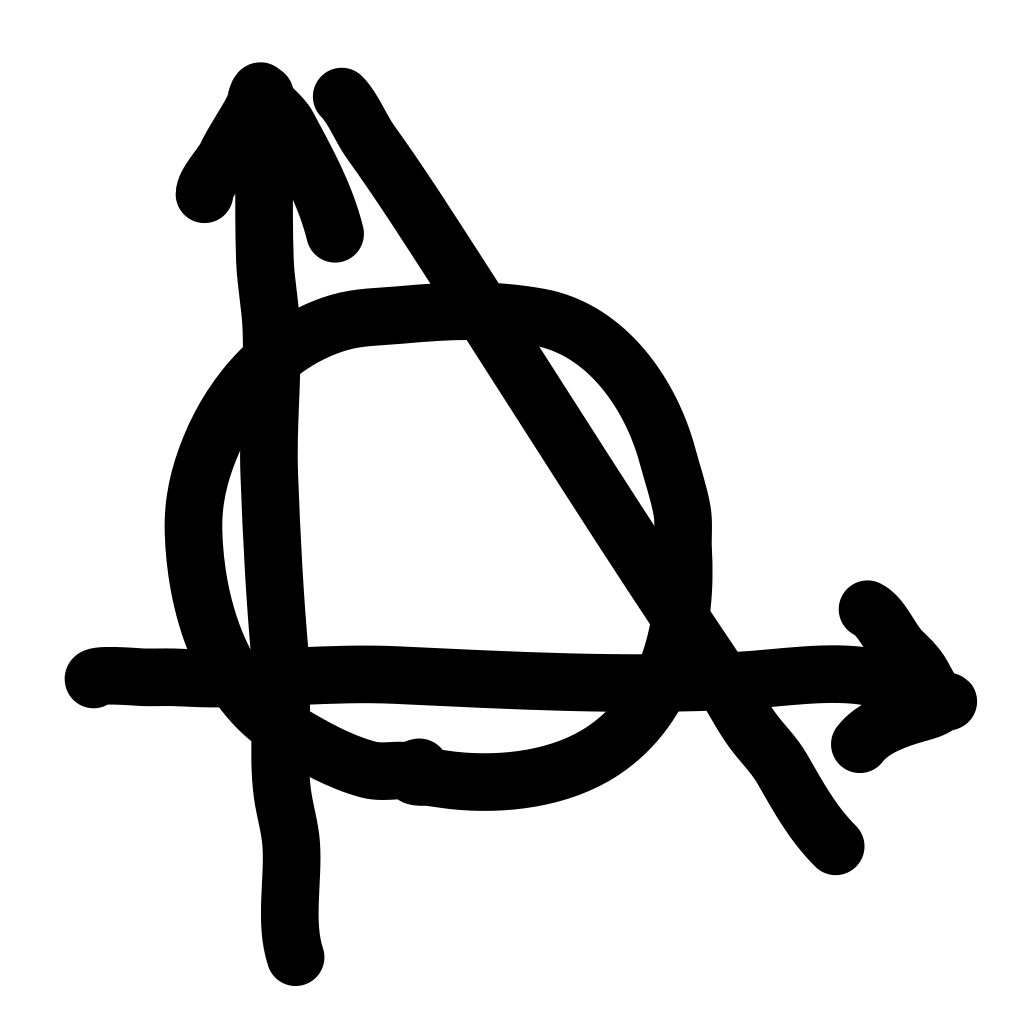
\includegraphics[width=8cm,bb=0 0 1920 1080]{./youtube/thumbnails/templates/smart_background/図形と方程式.jpeg}}
\at(6.6cm,0.2cm){\small\color{bradorange}$\overset{\text{図形と方程式}}{\text{応用}}$}
{\color{orange}\huge\underline{円の通過領域}}\vspace{0.3zw}

\Large 
問.放物線$y=x^2$上を動く点$\text{P}$がある.$P$を中心とし$x$軸に接する円の内部が通過する範囲を図示せよ.


\newpage



\at(0cm,0cm){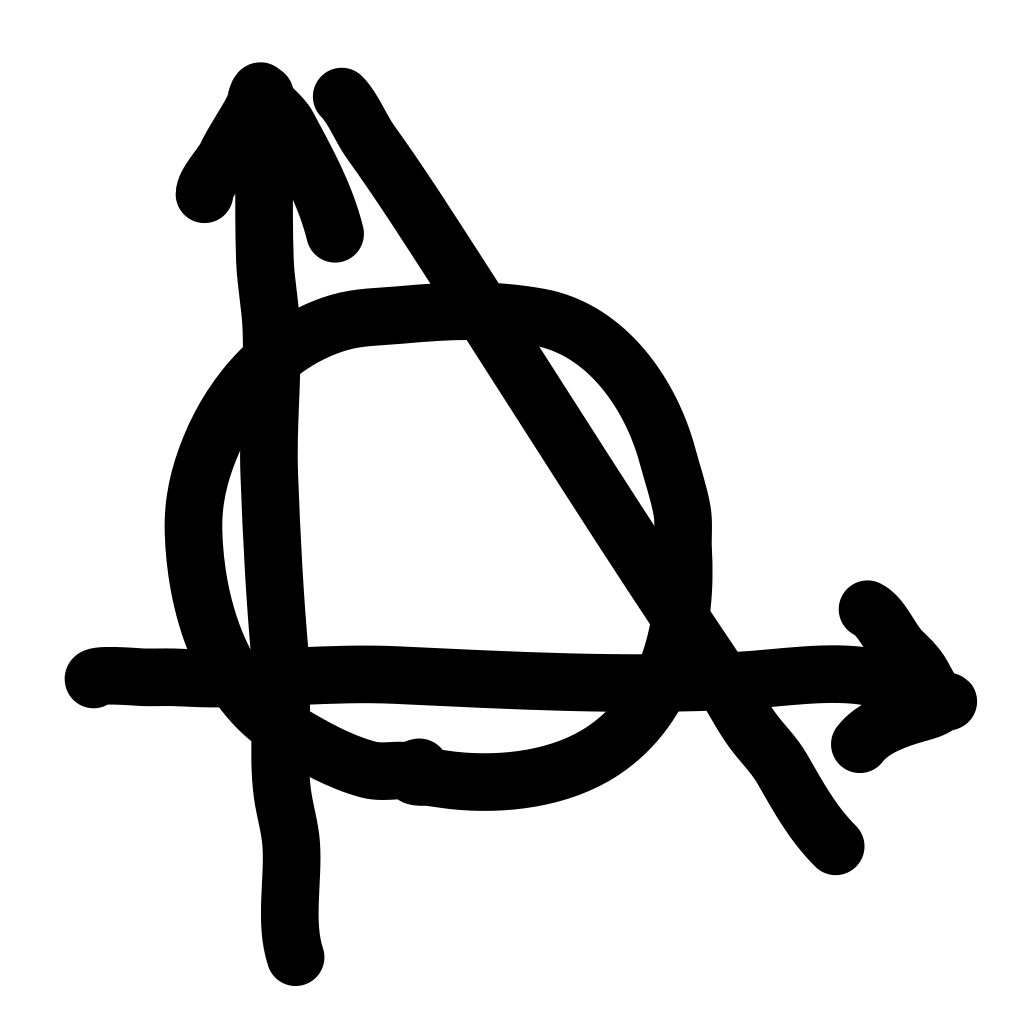
\includegraphics[width=8cm,bb=0 0 1920 1080]{./youtube/thumbnails/templates/smart_background/図形と方程式.jpeg}}
\at(6.6cm,0.2cm){\small\color{bradorange}$\overset{\text{図形と方程式}}{\text{応用}}$}
{\color{orange}\huge\underline{直線の通過領域}}\vspace{0.3zw}

\LARGE 
問.$t$が$t>0$の範囲を動くとき,直線$y=2tx-t^2$が通り得る領域を求めよ.


\newpage



\at(0cm,0cm){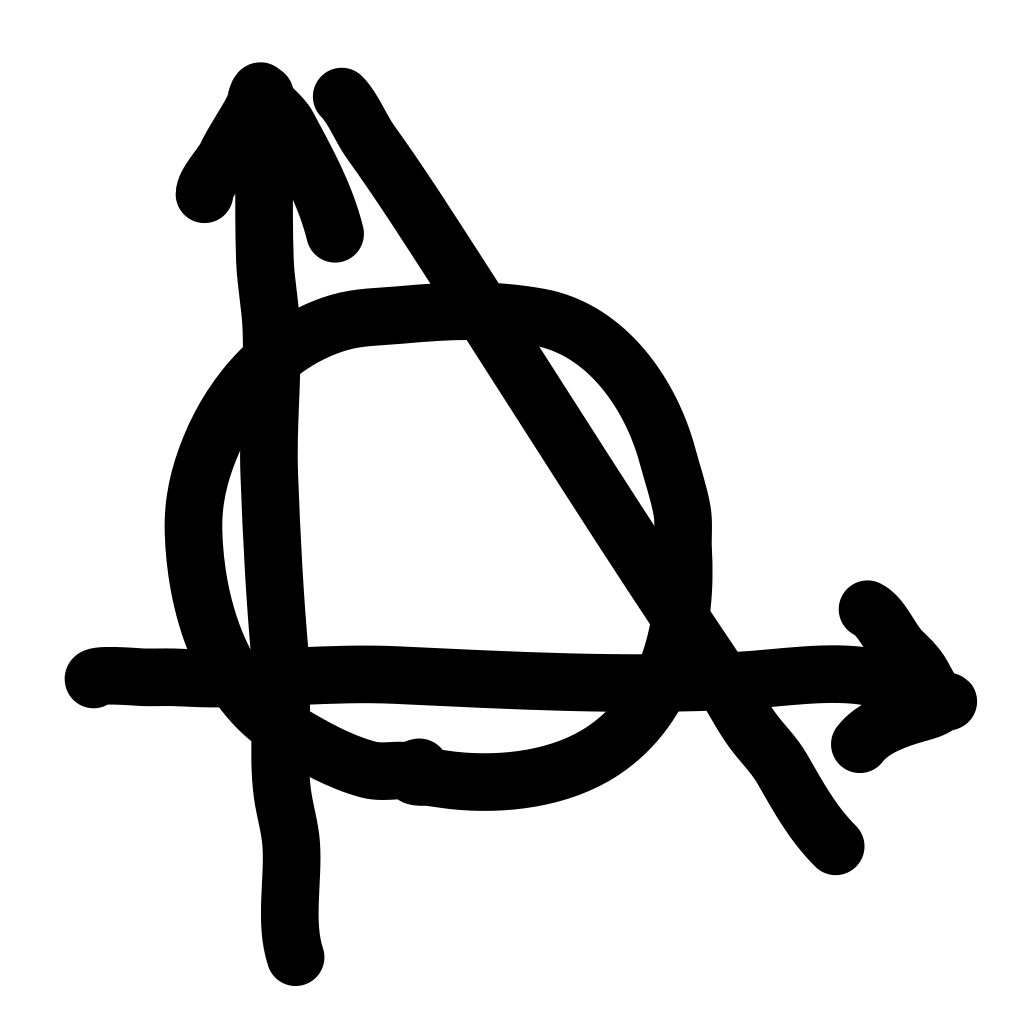
\includegraphics[width=8cm,bb=0 0 1920 1080]{./youtube/thumbnails/templates/smart_background/図形と方程式.jpeg}}
\at(6.6cm,0.2cm){\small\color{bradorange}$\overset{\text{図形と方程式}}{\text{応用}}$}
{\color{orange}\Large\underline{点$\left(\alpha +\beta ,\;\alpha \beta \right)$の動く範囲}}\vspace{0.3zw}

\Large 
問.点$\text{P}\left(\alpha ,\;\beta \right)$が$\alpha ^2+\beta ^2<1$を満たして動くとき,点$\text{Q}\left(\alpha +\beta ,\;\alpha \beta \right)$の動く範囲を図示せよ.


\newpage



\at(0cm,0cm){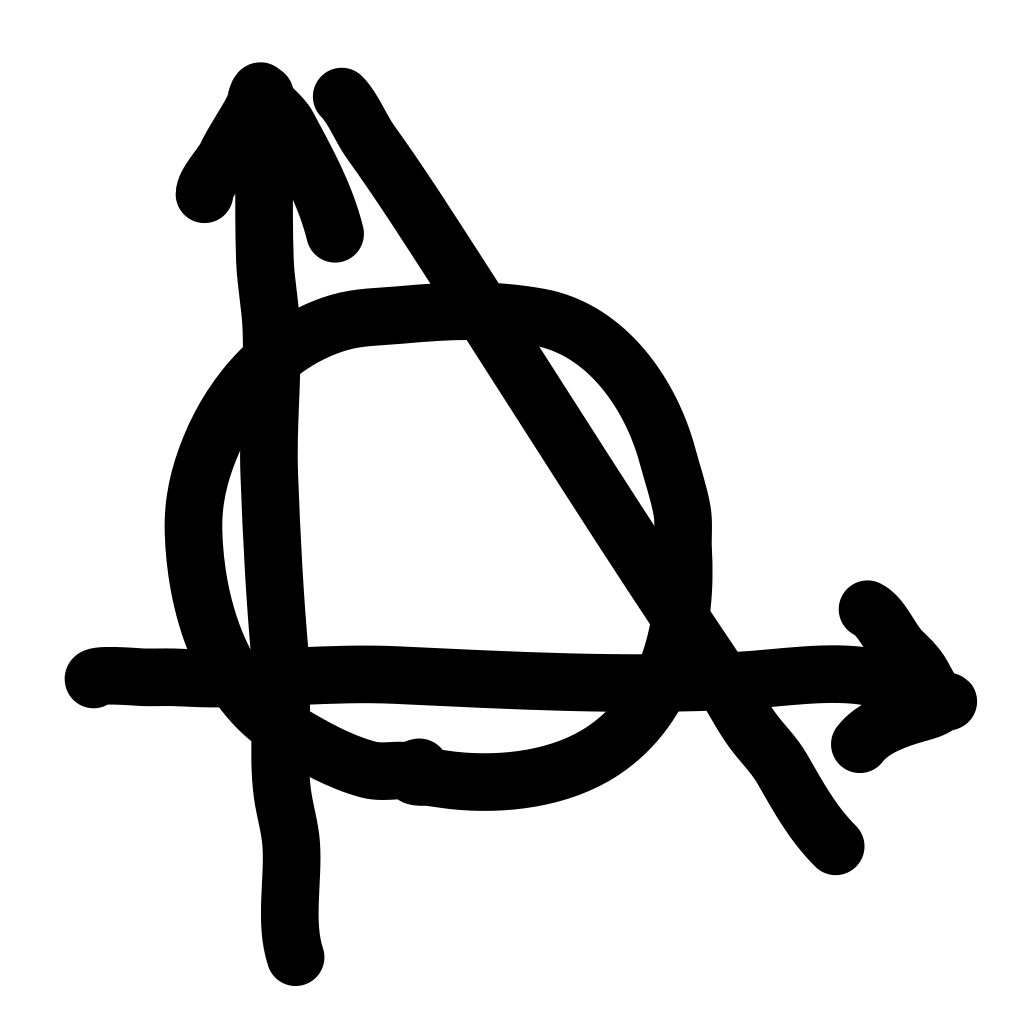
\includegraphics[width=8cm,bb=0 0 1920 1080]{./youtube/thumbnails/templates/smart_background/図形と方程式.jpeg}}
\at(6.6cm,0.2cm){\small\color{bradorange}$\overset{\text{図形と方程式}}{\text{応用}}$}
{\color{orange}\Large\underline{片側が動く線分の中点の軌跡}}\vspace{0.3zw}

\Large 
問.円$x^2+y^2=1$上の動点$\text{P}$と,点$\text{A}\left(3,\;4\right)$とを結ぶ線分の中点$\text{M}$の軌跡を求めよ.


\newpage



\at(0cm,0cm){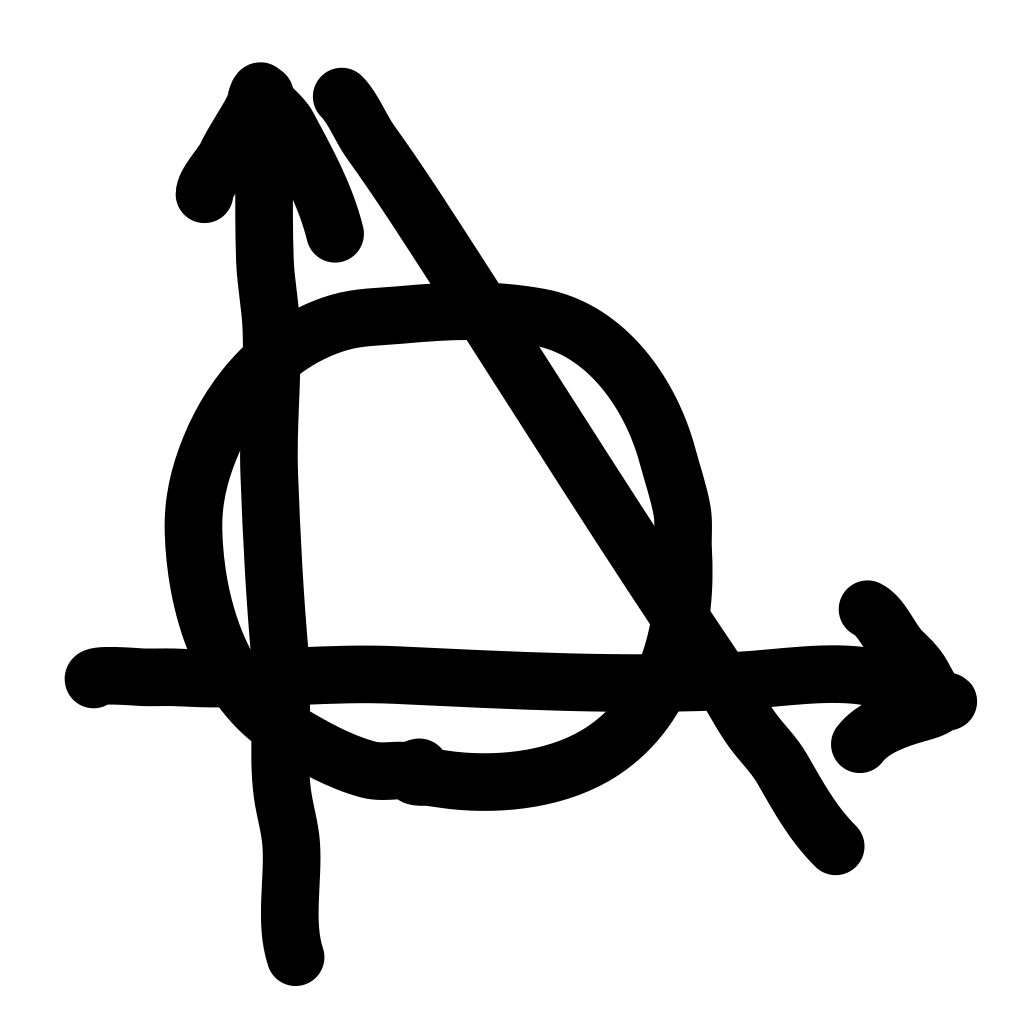
\includegraphics[width=8cm,bb=0 0 1920 1080]{./youtube/thumbnails/templates/smart_background/図形と方程式.jpeg}}
\at(6.6cm,0.2cm){\small\color{bradorange}$\overset{\text{図形と方程式}}{\text{応用}}$}
{\color{orange}\LARGE\underline{線形計画法 Lv.2 }}\vspace{0.3zw}

\large 
問.実数$x,\;y$が

\vspace{0.3zw}
\hspace{0.5zw}$x^2+y^2=2,\;x\geqq 0,\;y\geqq 0\vspace{0.3zw}$


を満たして変わるとき,$z=x+y$の最大値,最小値を求めよ.


\newpage



\at(0cm,0cm){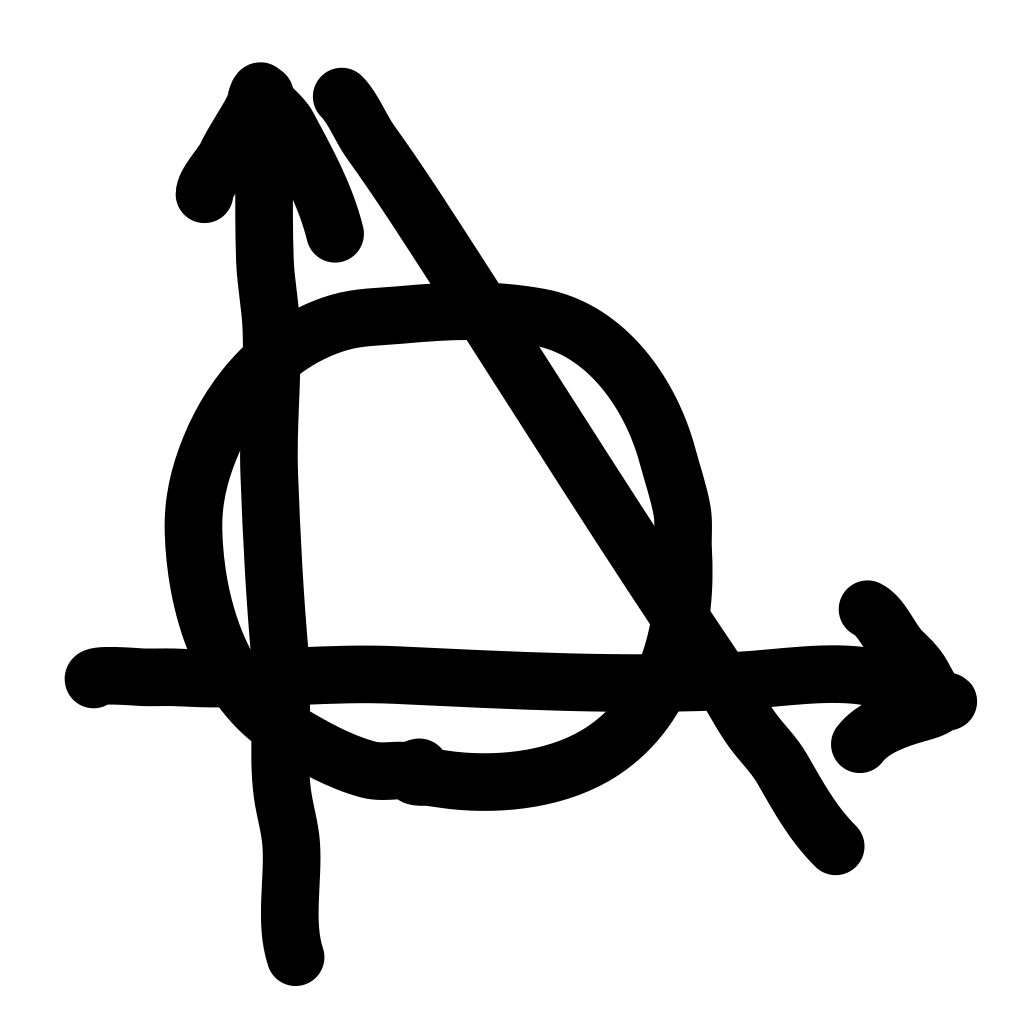
\includegraphics[width=8cm,bb=0 0 1920 1080]{./youtube/thumbnails/templates/smart_background/図形と方程式.jpeg}}
\at(6.6cm,0.2cm){\small\color{bradorange}$\overset{\text{図形と方程式}}{\text{応用}}$}
{\color{orange}\LARGE\underline{線形計画法 Lv.1 }}\vspace{0.3zw}

\normalsize 
問.実数$x,\;y$が条件

\vspace{0.3zw}
\hspace{0.5zw}$\left\{\begin{array}{l}x\geqq 0,\;y\geqq 0,\;\\ 2x+y\leqq 4,\;\\ x+4y\leqq 6,\;\\ 2x+3y\leqq 6\end{array}\right.\vspace{0.3zw}$


を満たして動くとき,$z=x+y$の最大値を求めよ.


\newpage



\at(0cm,0cm){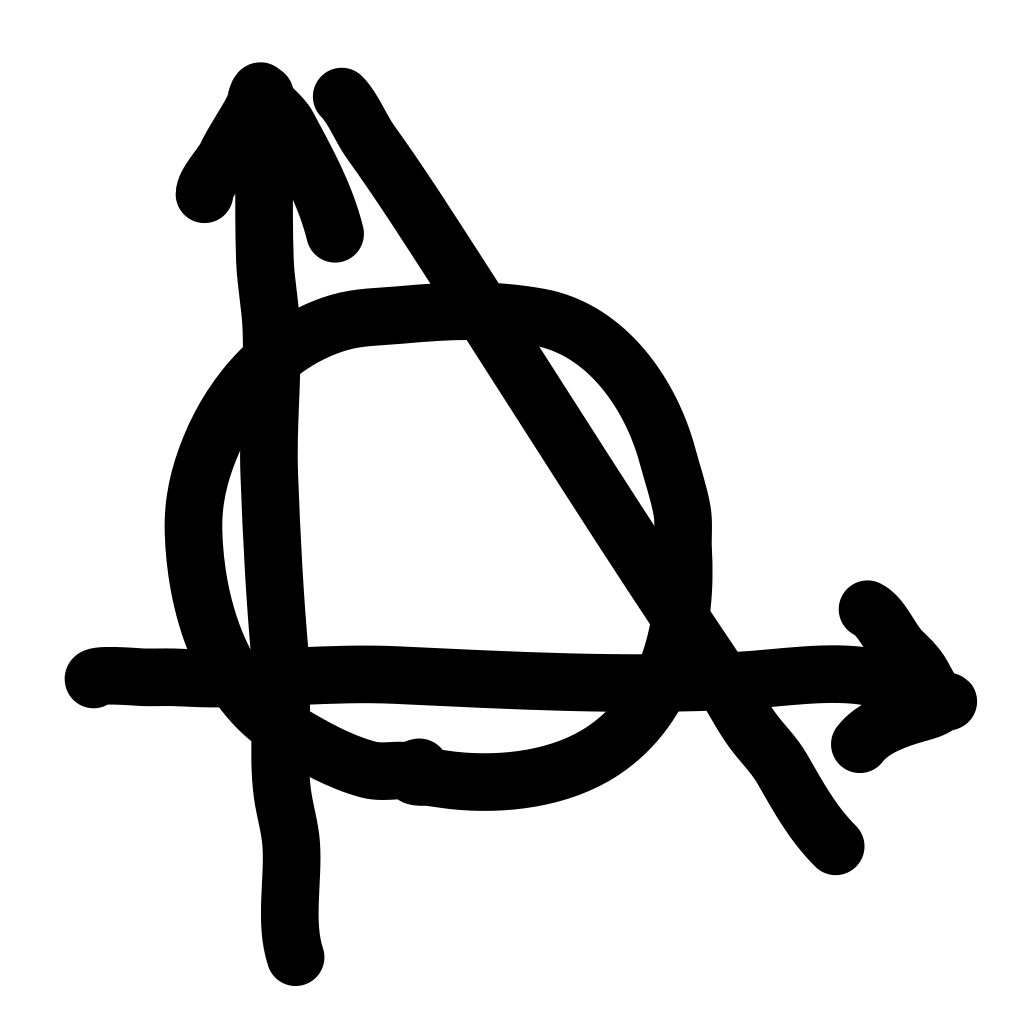
\includegraphics[width=8cm,bb=0 0 1920 1080]{./youtube/thumbnails/templates/smart_background/図形と方程式.jpeg}}
\at(6.6cm,0.2cm){\small\color{bradorange}$\overset{\text{図形と方程式}}{\text{応用}}$}
{\color{orange}\Large\underline{因数分解された不等式の領域}}\vspace{0.3zw}

\large 
問.次のおのおのの条件を満たす点$\left(x,\;y\right)$の存在範囲を図示せよ.\\
(1)  $\left(3x-y-5\right)\left(x^2+y^2-{25}\right)\leqq 0$\\
(2)  $\left(\zettaiti{x}+\zettaiti{y}-1\right)\left(x^2+y^2-1\right)<0$\\



\newpage



\at(0cm,0cm){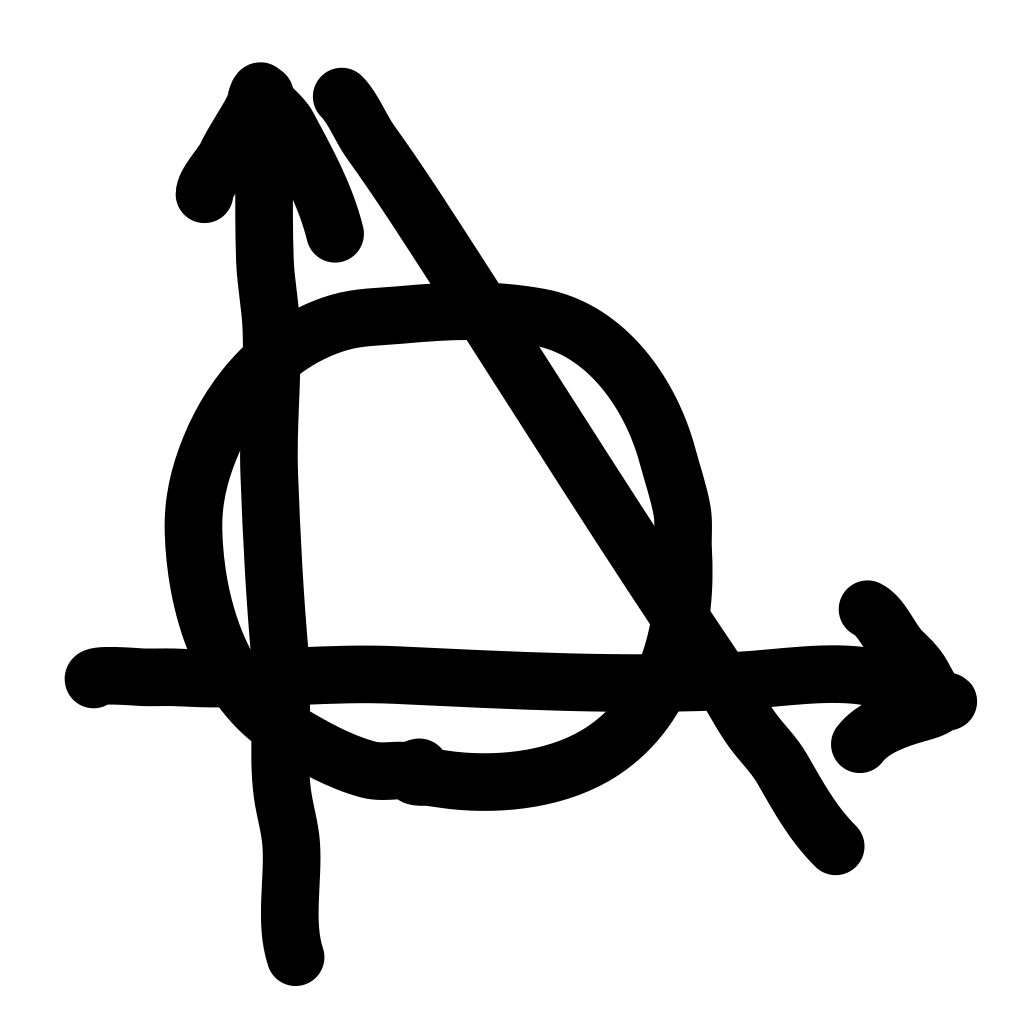
\includegraphics[width=8cm,bb=0 0 1920 1080]{./youtube/thumbnails/templates/smart_background/図形と方程式.jpeg}}
\at(6.6cm,0.2cm){\small\color{bradorange}$\overset{\text{図形と方程式}}{\text{応用}}$}
{\color{orange}\huge\underline{$2$直線の交点の軌跡}}\vspace{0.3zw}

\normalsize 
問.$t$がすべての実数値を取りながら変化するとき,$xy$平面上の$2$つの直線

\vspace{0.3zw}
\hspace{0.5zw}$\left\{\begin{array}{l}tx-y=t,\;\\ x+ty-2t-1=0\end{array}\right.\vspace{0.3zw}$


の交点の軌跡を求めよ.


\newpage



\at(0cm,0cm){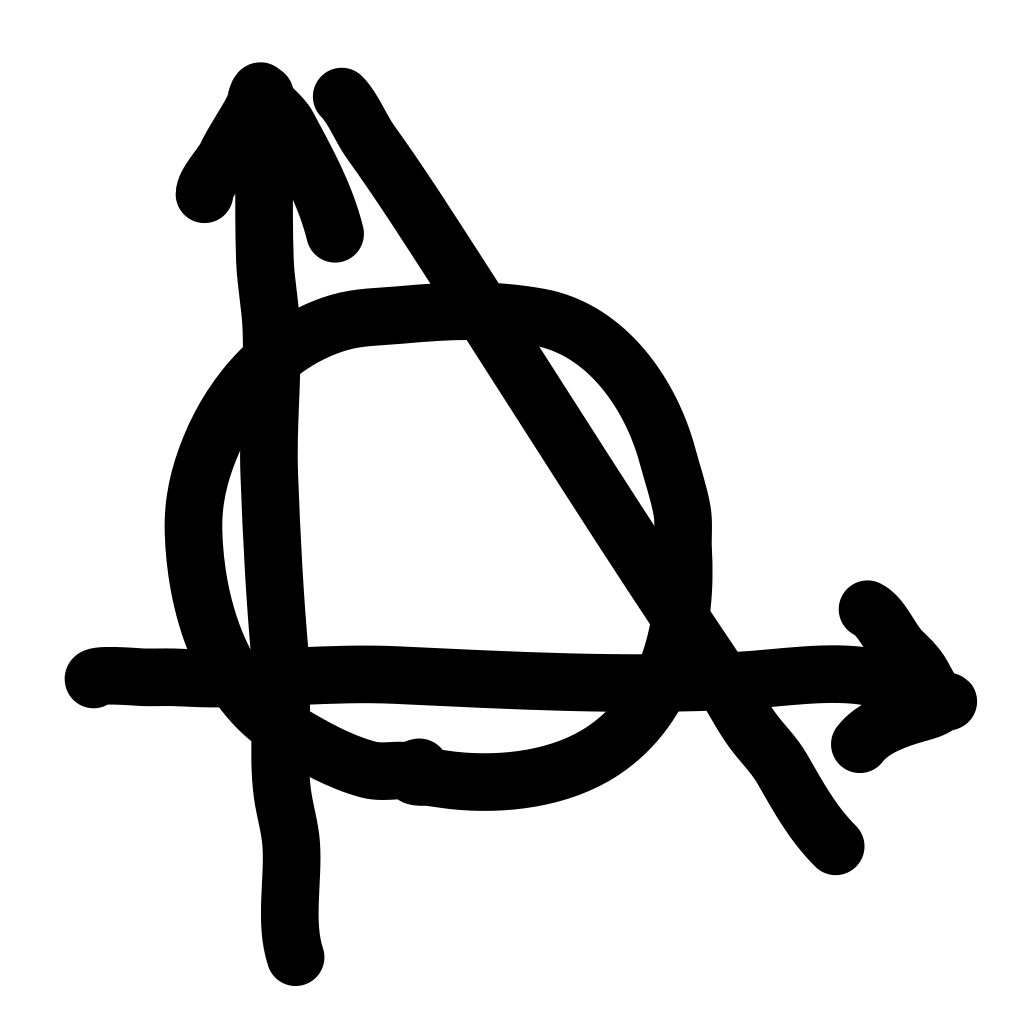
\includegraphics[width=8cm,bb=0 0 1920 1080]{./youtube/thumbnails/templates/smart_background/図形と方程式.jpeg}}
\at(6.6cm,0.2cm){\small\color{bradorange}$\overset{\text{図形と方程式}}{\text{応用}}$}
{\color{orange}\large\underline{放物線の直交する$2$接線の交点の軌跡}}\vspace{0.3zw}

\Large 
問.放物線$y=x^2$の異なる$2$接線が直交するとき,この$2$接線の交点$\text{P}$の軌跡を求めよ.


\newpage



\at(0cm,0cm){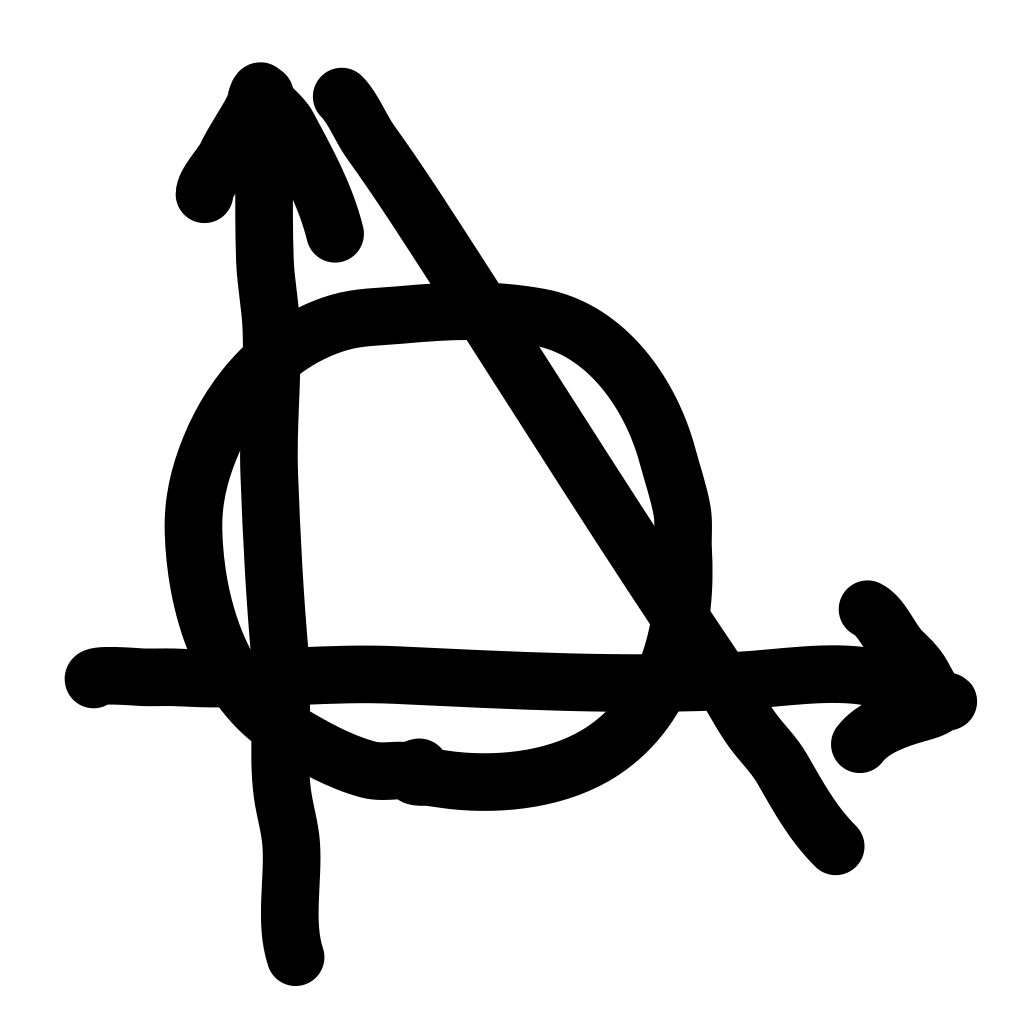
\includegraphics[width=8cm,bb=0 0 1920 1080]{./youtube/thumbnails/templates/smart_background/図形と方程式.jpeg}}
\at(6.6cm,0.2cm){\small\color{bradorange}$\overset{\text{図形と方程式}}{\text{応用}}$}
{\color{orange}\Large\underline{2交点の中点の軌跡 Lv.2}}\vspace{0.3zw}



\small 
問.円$C:x^2+y^2=1$と直線$l:y=m\left(x-2\right)$が\\
\hspace{0.2zw}異なる$2$点で交わるように$m$の値が変化するとき,

\huge
\vspace{-0.2zw}
\hspace{0.2zw}円$C$と直線$l$の\vspace{-0.0zw}\\
\hfill 2交点の中点$\text{M}$の軌跡\hspace{0.4zw}

\small
\vspace{0.2zw}
\hfill を求めよ.


\newpage



\at(0cm,0cm){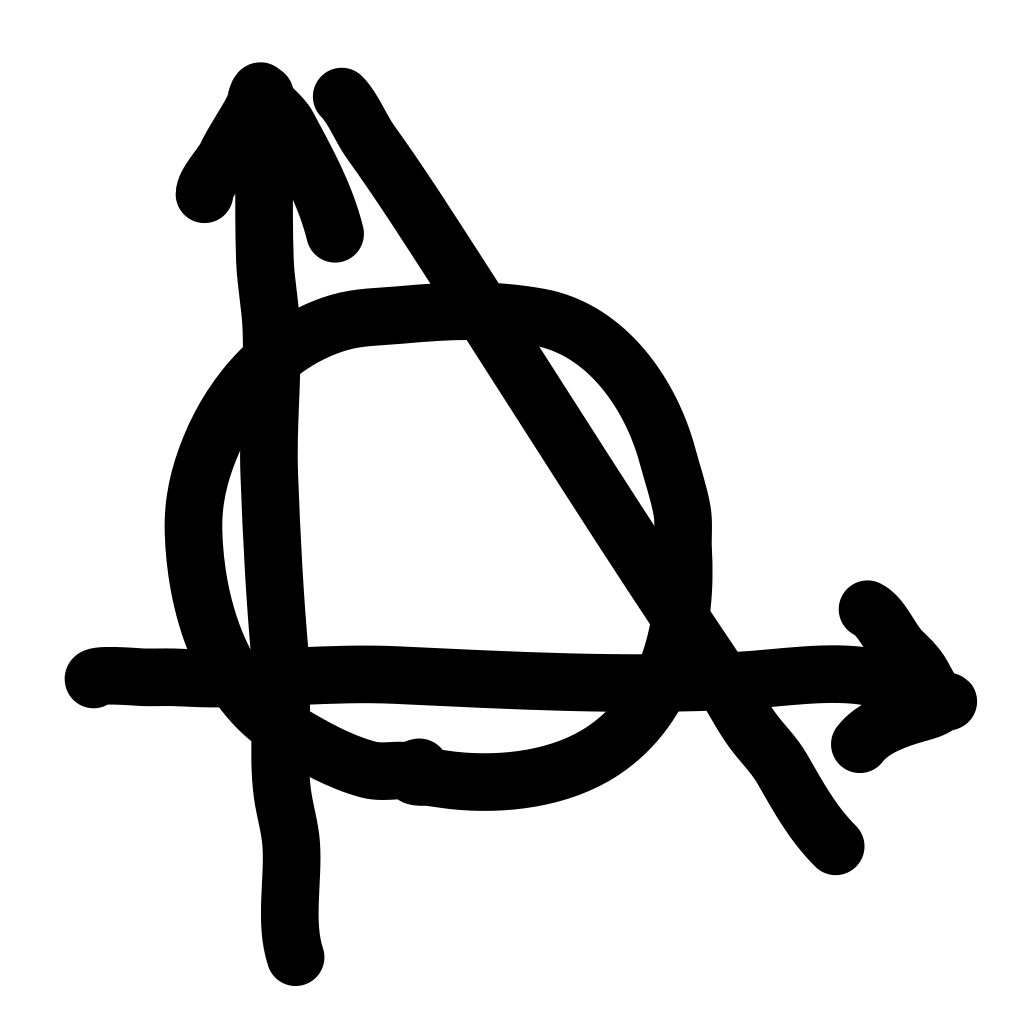
\includegraphics[width=8cm,bb=0 0 1920 1080]{./youtube/thumbnails/templates/smart_background/図形と方程式.jpeg}}
\at(6.6cm,0.2cm){\small\color{bradorange}$\overset{\text{図形と方程式}}{\text{応用}}$}
{\color{orange}\huge\underline{軌跡の除去点}}\vspace{0.3zw}

\normalsize 
問.変数$t$が全ての実数値をとって変化するとき,次式で定まる点$\text{P}\left(x,\;y\right)$の描く軌跡を求めよ.

\LARGE
\vspace{0.6zw}
\hspace{0.1zw}$x=\bunsuu{1}{{}t^2+1},\;y=\bunsuu{t}{{}t^2+1}\vspace{0.3zw}$




\newpage



\at(0cm,0cm){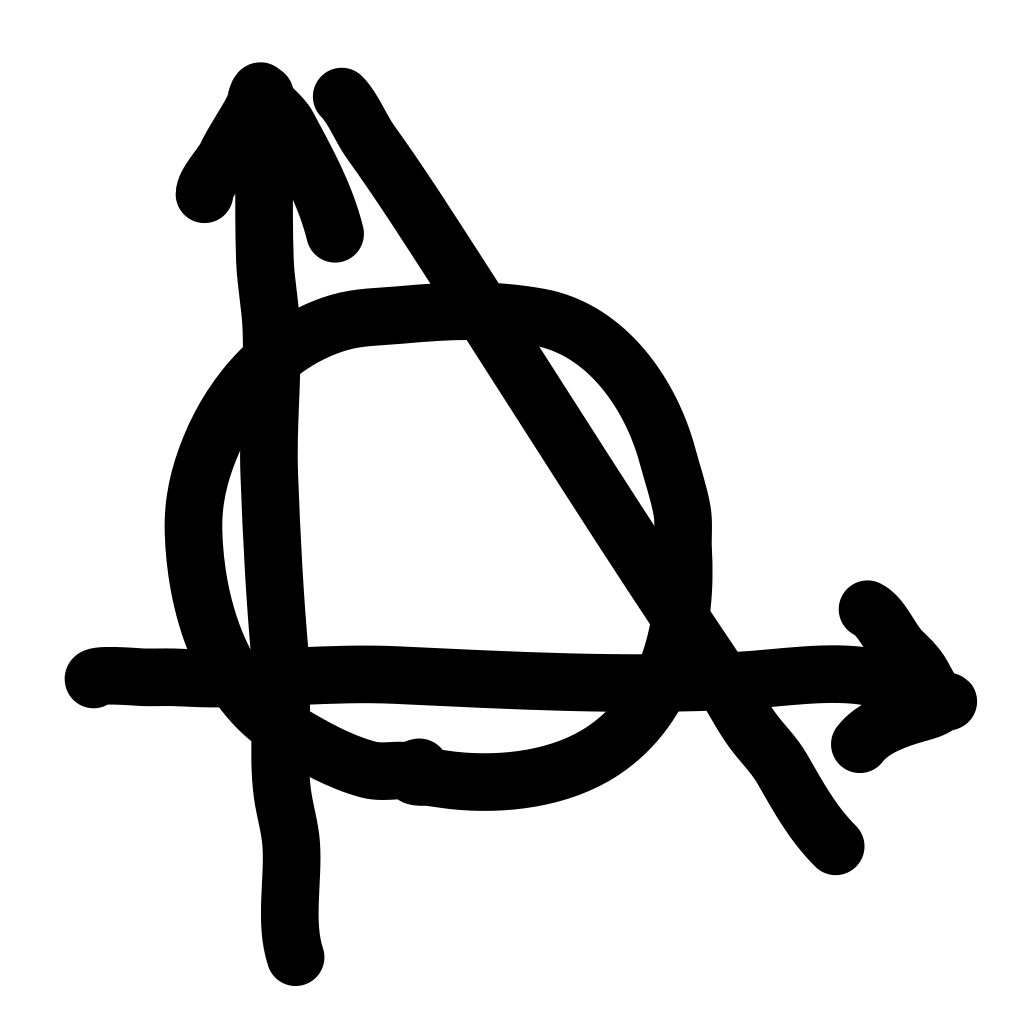
\includegraphics[width=8cm,bb=0 0 1920 1080]{./youtube/thumbnails/templates/smart_background/図形と方程式.jpeg}}
\at(6.6cm,0.2cm){\small\color{bradorange}$\overset{\text{図形と方程式}}{\text{応用}}$}
{\color{orange}\LARGE\underline{放物線の頂点の軌跡}}\vspace{0.3zw}

\large 
問.$m$が実数値を変化するとき,放物線

\huge
\vspace{-0.0zw}
\hspace{0.1zw}$y=x^2-2mx+2m$\vspace{-0.0zw}\\
\hfill の頂点の軌跡\hspace{0.4zw}

\large 
\vspace{0.2zw}
\hfill を求めよ.


\newpage



\at(0cm,0cm){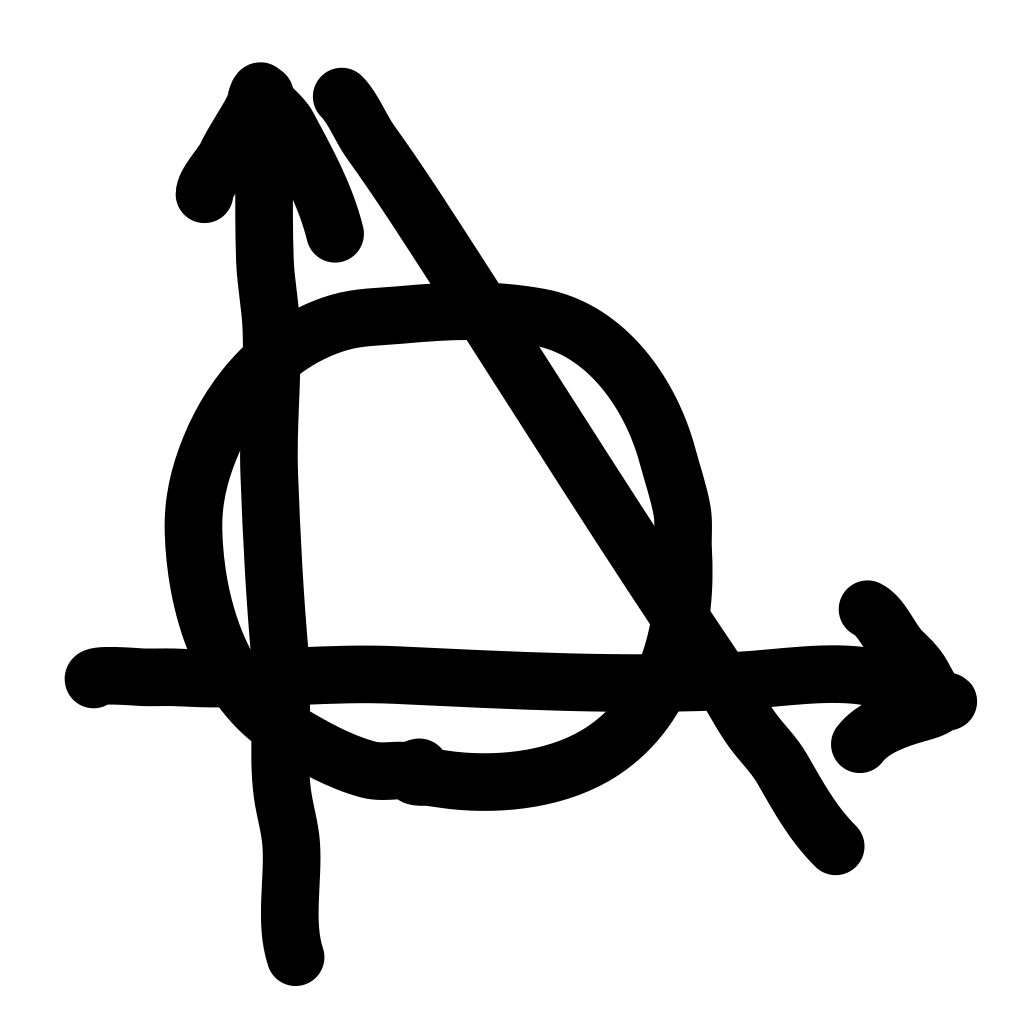
\includegraphics[width=8cm,bb=0 0 1920 1080]{./youtube/thumbnails/templates/smart_background/図形と方程式.jpeg}}
\at(6.6cm,0.2cm){\small\color{bradorange}$\overset{\text{図形と方程式}}{\text{応用}}$}
{\color{orange}\Large\underline{パラメータ表示された点の軌跡}}\vspace{0.3zw}

\normalsize 
問.変数$t$が全ての実数値をとって変化するとき,次のおのおの式で定められる点$\text{P}\left(x,\;y\right)$の描く軌跡を求め,図示せよ.\\
(1)  $x=t-1,\;y=t^2+4t-1$\\
(2)  $x=t^2-1,\;y=t^4+4t^2-1$\\



\newpage



\at(0cm,0cm){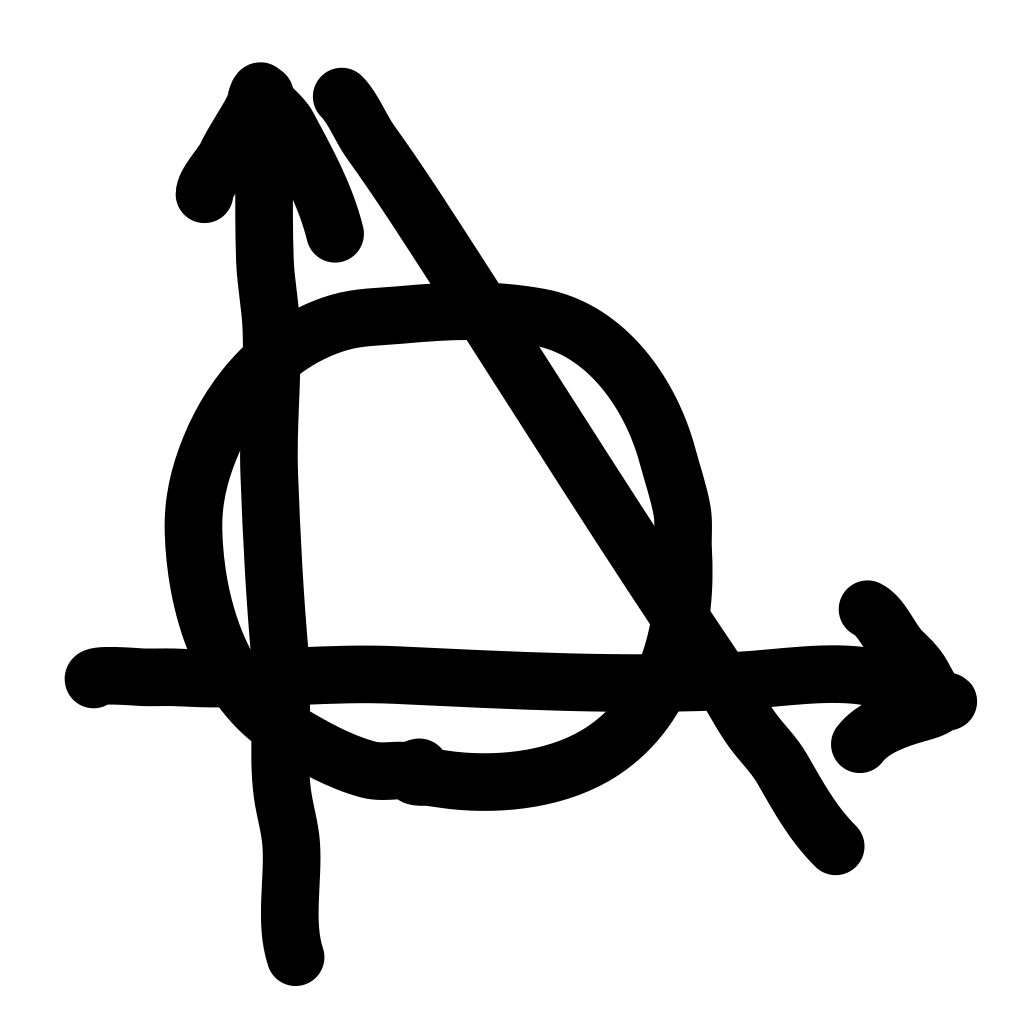
\includegraphics[width=8cm,bb=0 0 1920 1080]{./youtube/thumbnails/templates/smart_background/図形と方程式.jpeg}}
\at(6.6cm,0.2cm){\small\color{bradorange}$\overset{\text{図形と方程式}}{\text{応用}}$}
{\color{orange}\large\underline{$2$点からの距離の比が一定である点の軌跡}}\vspace{0.3zw}

\large 
問.$2$点$\text{A}\left(-3,\;0\right),\;\text{B}\left(3,\;0\right)$がある.

\huge
\vspace{-0.0zw}
\hspace{0.5zw}$\text{AP}:\text{BP}=2:1$\vspace{-0.0zw}\\
\hfill を満たす点$\text{P}$の軌跡\hspace{0.4zw}

\large 
\vspace{0.2zw}
\hfill を求めよ.


\newpage



\at(0cm,0cm){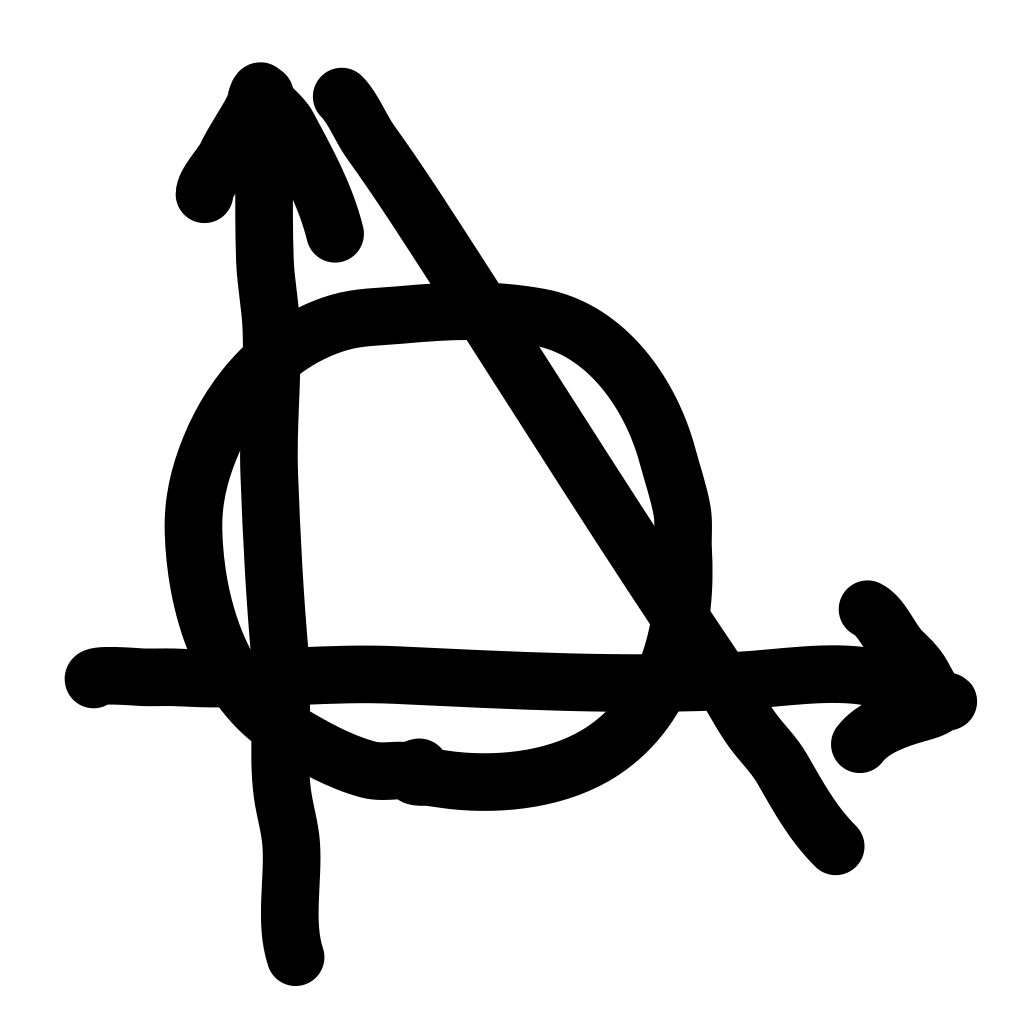
\includegraphics[width=8cm,bb=0 0 1920 1080]{./youtube/thumbnails/templates/smart_background/図形と方程式.jpeg}}
\at(6.6cm,0.2cm){\small\color{bradorange}$\overset{\text{図形と方程式}}{\text{応用}}$}
{\color{orange}\Large\underline{$2$点から等距離の点の軌跡}}\vspace{0.3zw}

\large 
問.$2$点$\text{A}\left(-1,\;3\right),\;\text{B}\left(2,\;1\right)$からの

\Huge
\vspace{-0.2zw}
\hspace{0.2zw}距離が等しい\vspace{-0.2zw}\\
\hfill 点$\text{P}$の軌跡\hspace{0.2zw}

\large 
\vspace{0.2zw}
\hfill を求めよ.


\end{document}

